%!TEX encoding=UTF-8 Unicode

% Layers

\definecolor{Computer}{HTML}{D95F02}
\definecolor{Science}{HTML}{1B9E77}
\definecolor{Theory}{HTML}{7570B3}

\tikzstyle{arr}  = [-latex,very thick]
\tikzset{
  filled box/.style = {
    shape = rectangle,
    draw  = #1,
    fill  = #1,
    text width=6em,
    centered,
    rounded corners},
}

%\newlength{\cornerlength}
%\setlength{\cornerlength}{.1}

\begin{tikzpicture}[font=\small,scale=1]
    \node[filled box=Computer] (computers)   at (0,3) {\only<5->{\textbf{More\newline performant\newline}} computers};
    \uncover<2->{
        \node[filled box=Science] (simu)        at (5,5) {\only<4->{\textbf{More complex\newline}} Simulation \newline and large scale \newline experiments};
        \path[arr,Computer] (computers.north) edge[out=90,in=180] (simu.west);
}
    \uncover<3->{
        \node[filled box=Theory] (th)          at (8,0)  {New theories};
        \path[arr,Science] (simu.east) edge[out=0,in=90] (th.north);
    }

    \uncover<4->{
        \path[arr,Theory] (th.west) edge[out=180,in=-75] (simu.south);
    }
 
    \uncover<5->{
        \path[arr,Science] (simu.south) edge[out=-105,in=0] (computers.east);
    }


\end{tikzpicture}
% vim: et si sta lbr  sw=4 ts=4 spelllang=en_us
